\documentclass[tikz,border=12pt]{standalone}
\usepackage[T1]{fontenc}
\usepackage{mathpazo}
\usepackage{amsmath,amssymb}
\usetikzlibrary{arrows.meta, positioning, calc, fit, patterns, decorations.pathreplacing}

\definecolor{stblue}{HTML}{7B97AD}
\definecolor{rwgold}{HTML}{B8995E}
\definecolor{sage}{HTML}{7A9A7E}
\definecolor{dkbrown}{HTML}{3D3530}
\definecolor{wmgray}{HTML}{7B7067}
\definecolor{cream}{HTML}{F9F6F0}
\definecolor{border}{HTML}{D4C9B8}
\definecolor{terracotta}{HTML}{C47A6A}
\definecolor{lavender}{HTML}{907EA0}

\begin{document}
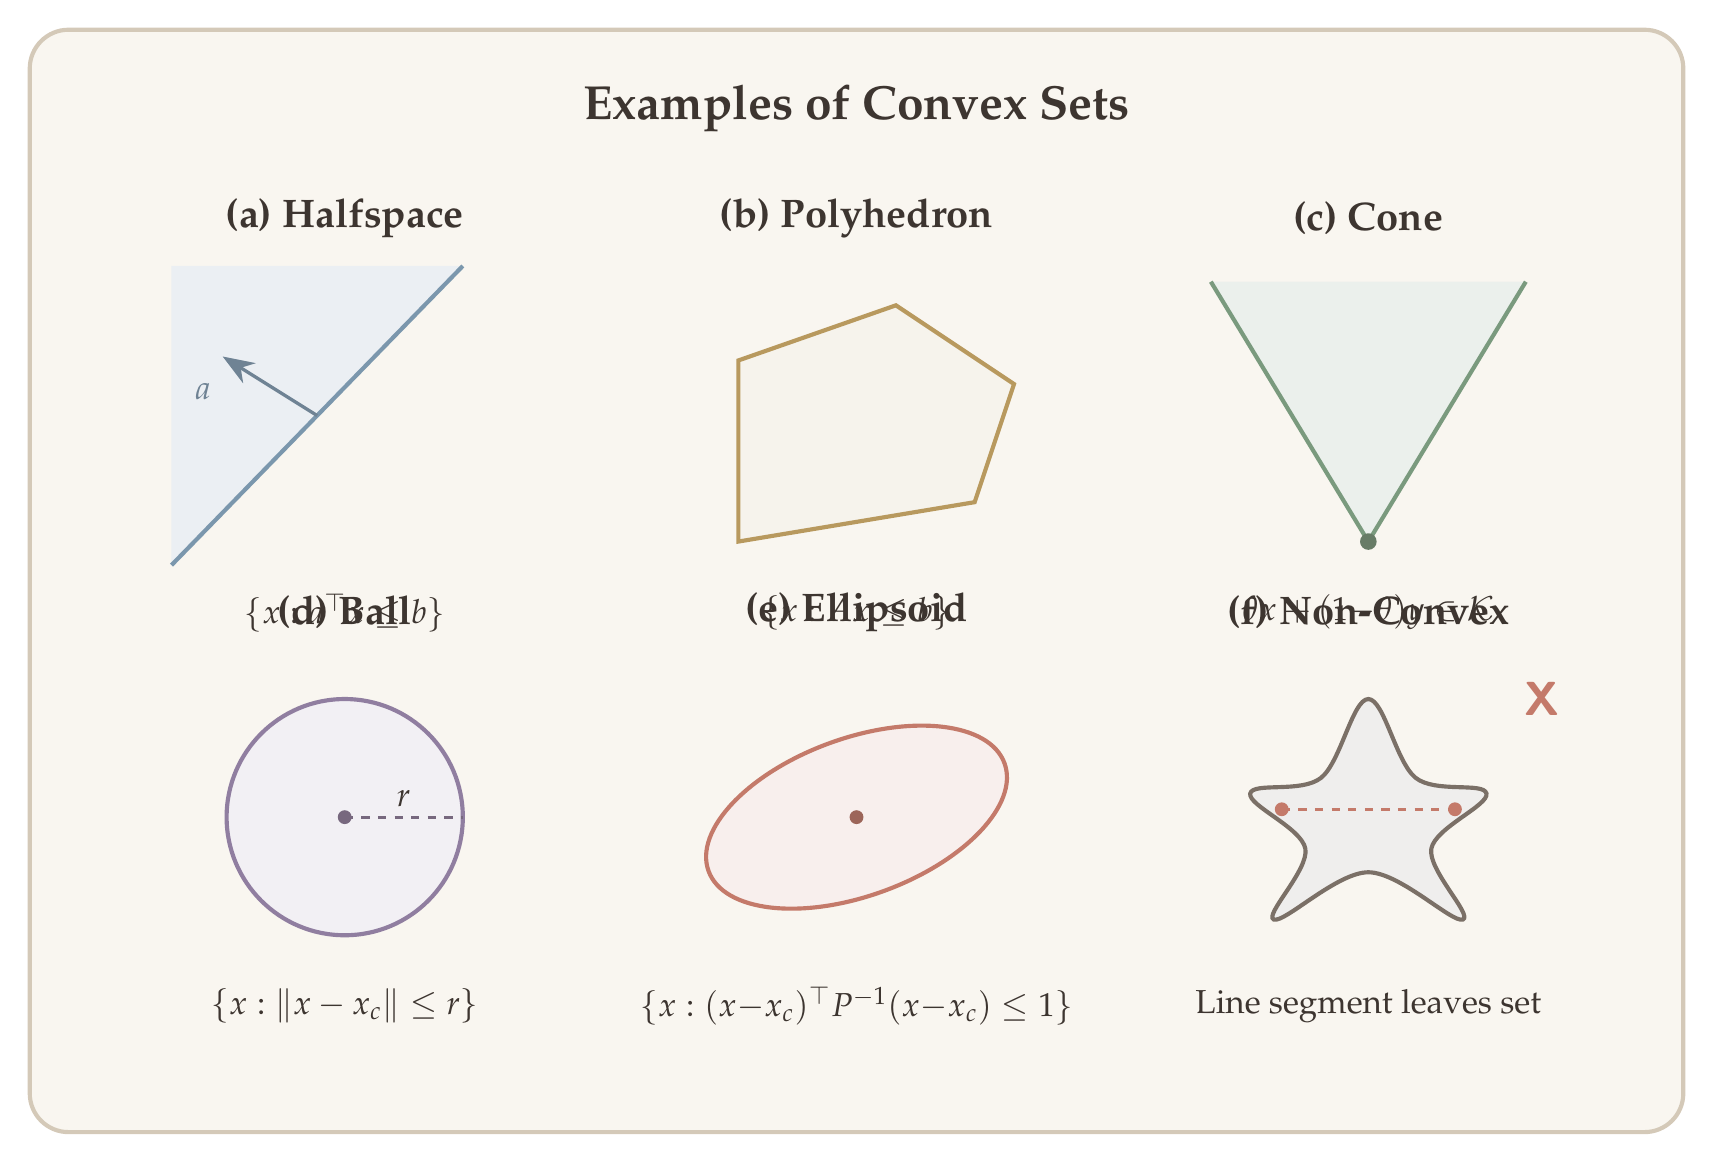
\begin{tikzpicture}[>={Stealth[length=4mm, width=3mm]}, line width=1.5pt]

% Background
\fill[cream, rounded corners=14pt] (-0.5,-0.5) rectangle (20.5,13.5);
\draw[border, line width=1.5pt, rounded corners=14pt] (-0.5,-0.5) rectangle (20.5,13.5);

% Title
\node[font=\LARGE\bfseries, text=dkbrown] at (10,12.5) {Examples of Convex Sets};

% Grid layout: 3 columns x 2 rows
% Column centers: 3.5, 10, 16.5
% Row centers: 8.5, 3.5

% --- (a) Halfspace ---
\begin{scope}[shift={(3.5,8.5)}]
  \node[font=\Large\bfseries, text=dkbrown] at (0,2.6) {(a) Halfspace};
  % Shaded halfspace
  \fill[stblue!15] (-2.2,-1.8) -- (1.5,2) -- (-2.2,2) -- cycle;
  % Boundary line
  \draw[stblue, line width=1.5pt] (-2.2,-1.8) -- (1.5,2);
  % Normal arrow
  \draw[->, stblue!80!dkbrown, line width=1.2pt] (-0.35,0.1) -- (-1.55,0.85);
  \node[font=\large, text=stblue!80!dkbrown] at (-1.8,0.4) {$a$};
  % Label
  \node[font=\large, text=dkbrown] at (0,-2.4) {$\{x : a^\top x \leq b\}$};
\end{scope}

% --- (b) Polyhedron ---
\begin{scope}[shift={(10,8.5)}]
  \node[font=\Large\bfseries, text=dkbrown] at (0,2.6) {(b) Polyhedron};
  \fill[rwgold!12] (-1.5,-1.5) -- (1.5,-1) -- (2,0.5) -- (0.5,1.5) -- (-1.5,0.8) -- cycle;
  \draw[rwgold, line width=1.5pt] (-1.5,-1.5) -- (1.5,-1) -- (2,0.5) -- (0.5,1.5) -- (-1.5,0.8) -- cycle;
  \node[font=\large, text=dkbrown] at (0,-2.4) {$\{x : Ax \leq b\}$};
\end{scope}

% --- (c) Cone ---
\begin{scope}[shift={(16.5,8.5)}]
  \node[font=\Large\bfseries, text=dkbrown] at (0,2.6) {(c) Cone};
  \fill[sage!15] (0,-1.5) -- (-2,1.8) -- (2,1.8) -- cycle;
  \draw[sage, line width=1.5pt] (0,-1.5) -- (-2,1.8);
  \draw[sage, line width=1.5pt] (0,-1.5) -- (2,1.8);
  \fill[sage!70!dkbrown] (0,-1.5) circle (3pt);
  \node[font=\large, text=dkbrown] at (0,-2.4) {$\theta x + (1{-}\theta)y \in \mathcal{K}$};
\end{scope}

% --- (d) Ball ---
\begin{scope}[shift={(3.5,3.5)}]
  \node[font=\Large\bfseries, text=dkbrown] at (0,2.6) {(d) Ball};
  \fill[lavender!12] (0,0) circle (1.5);
  \draw[lavender, line width=1.5pt] (0,0) circle (1.5);
  \fill[lavender!70!dkbrown] (0,0) circle (2.5pt);
  \draw[lavender!70!dkbrown, line width=1pt, dashed] (0,0) -- (1.5,0) node[midway, above, font=\large, text=dkbrown] {$r$};
  \node[font=\large, text=dkbrown] at (0,-2.4) {$\{x : \|x - x_c\| \leq r\}$};
\end{scope}

% --- (e) Ellipsoid ---
\begin{scope}[shift={(10,3.5)}]
  \node[font=\Large\bfseries, text=dkbrown] at (0,2.6) {(e) Ellipsoid};
  \fill[terracotta!12, rotate=20] (0,0) ellipse (2 and 1);
  \draw[terracotta, line width=1.5pt, rotate=20] (0,0) ellipse (2 and 1);
  \fill[terracotta!70!dkbrown] (0,0) circle (2.5pt);
  \node[font=\large, text=dkbrown] at (0,-2.4) {$\{x : (x{-}x_c)^\top P^{-1}(x{-}x_c) \leq 1\}$};
\end{scope}

% --- (f) Non-convex ---
\begin{scope}[shift={(16.5,3.5)}]
  \node[font=\Large\bfseries, text=dkbrown] at (0,2.6) {(f) Non-Convex};
  % Star/non-convex shape
  \fill[wmgray!12] plot[smooth cycle, tension=0.6] coordinates {
    (0,1.5) (0.6,0.5) (1.5,0.3) (0.8,-0.4) (1.2,-1.3) (0,-0.7) (-1.2,-1.3) (-0.8,-0.4) (-1.5,0.3) (-0.6,0.5)
  };
  \draw[wmgray, line width=1.5pt] plot[smooth cycle, tension=0.6] coordinates {
    (0,1.5) (0.6,0.5) (1.5,0.3) (0.8,-0.4) (1.2,-1.3) (0,-0.7) (-1.2,-1.3) (-0.8,-0.4) (-1.5,0.3) (-0.6,0.5)
  };
  % Line segment showing non-convexity
  \draw[terracotta, line width=1.2pt, dashed] (-1.1,0.1) -- (1.1,0.1);
  \fill[terracotta] (-1.1,0.1) circle (2.5pt);
  \fill[terracotta] (1.1,0.1) circle (2.5pt);
  % X mark
  \node[font=\LARGE\bfseries, text=terracotta] at (2.2,1.5) {\textsf{X}};
  \node[font=\large, text=dkbrown] at (0,-2.4) {Line segment leaves set};
\end{scope}

\end{tikzpicture}
\end{document}
